\documentclass[8pt]{beamer}
\usepackage{tikz}
\usepackage[utf8]{vietnam}
\usepackage{amsmath}
\usepackage{graphicx}
\usepackage{wrapfig}
\usepackage{hyperref}
\usepackage{mathrsfs}
\usepackage{verbatim}
\usepackage{algorithm}
\usepackage{algpseudocode}
\usetheme{Copenhagen}
\usecolortheme{dolphin}
\setbeamertemplate{navigation symbols}{}
\setbeamertemplate{headline}{}
\title[Chương 5: Thiết kế bộ lọc FIR] %optional
{Chương 5: Thiết kế bộ lọc FIR}
\subtitle{Xử lý tín hiệu số}
\author[Xử lý tín hiệu số] % (optional)
{Tín Vũ}
\date[VLC 2021] % (optional)
{tinvu1309@gmail.com}
\begin{document}
\frame{\titlepage}
\begin{frame}{Mục lục}
	\tableofcontents
\end{frame}
\begin{frame}{Giới thiệu playlist}
	\section{Giới thiệu playlist}
	\begin{itemize}
		\item Mình là Tín Vũ, hiện đang là sinh viên học tại Trường Đại học Công nghệ, Đại học Quốc gia Hà Nội. Mình tạo playlist video này để hỗ trợ các bạn học môn \textbf{Xử lý tín hiệu số}.
		\item Khác với môn học tiên quyết \alert{Tín hiệu hệ thống} trước đó, bài giảng môn học này \textbf{hoàn toàn bám sát với đề cương và giáo trình nội bộ} của trường mình, nên các bạn trường khác cần phải lưu ý rất kĩ điều này.
		\item Không chỉ dừng lại ở lý thuyết, playlist này \textbf{có bổ sung hướng dẫn lập trình cơ bản bằng GNU Octave/Matlab} để vẽ phổ tín hiệu, đáp ứng tần số và thiết kế bộ lọc.
		\item Môn học này bao gồm \textbf{6 chương}, các chương đều liên quan rất chặt chẽ với nhau nên hãy học cẩn thận ngay từ \alert{Chương 0} để ôn thi cuối kì đỡ vất vả.
	\end{itemize}
\end{frame}
\begin{frame}{Tài liệu tham khảo}
	\section{Tài liệu tham khảo}
	\begin{itemize}
		\item Tài liệu tham khảo chính: Giáo trình Xử lý tín hiệu số (Nguyễn Linh Trung, Trần Đức Tân, Huỳnh Hữu Tuệ, ĐHCN, 2012).
		\item Tài liệu tham khảo phụ: Discrete-time Signal Processing (Alan V.Oppenheim, 2nd edition).
	\end{itemize}
\end{frame}
\begin{frame}{Quy trình xử lý tín hiệu số}
	\section{Quy trình xử lý tín hiệu số}
	\begin{figure}[h]
		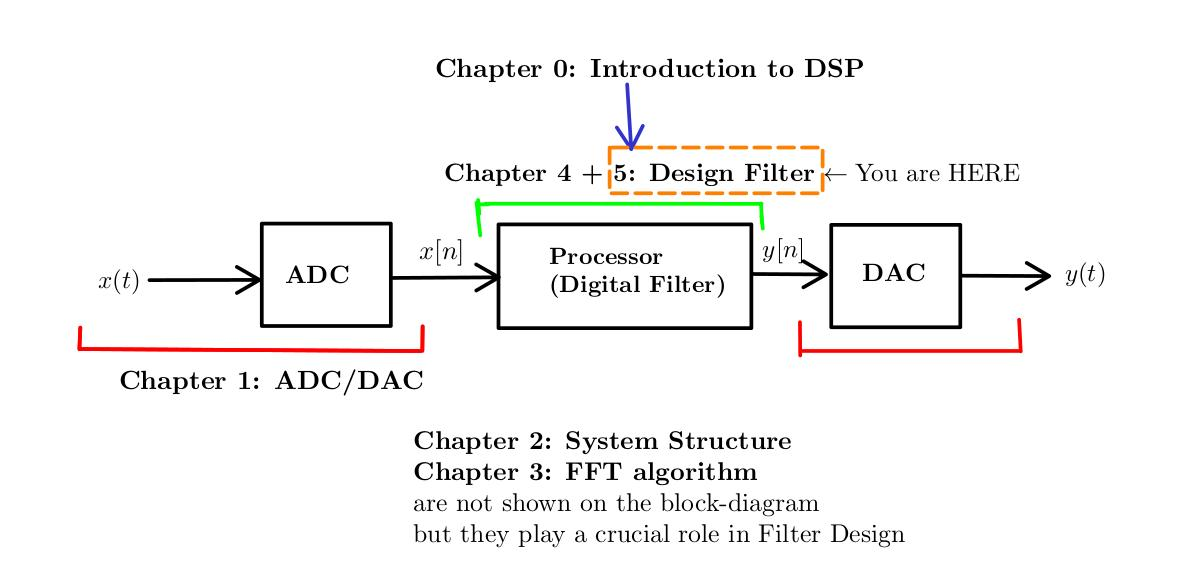
\includegraphics[width=1.1\textwidth]{1.jpg}
		\caption{DSP Learning Process}			\label{fig:re1}
	\end{figure}

\end{frame}
\begin{frame}{Ý tưởng thiết kế bộ lọc FIR}
	\section{Ý tưởng thiết kế bộ lọc FIR}
	Nhược điểm lớn nhất của bộ lọc IIR đó là \textbf{méo pha phi tuyến}, nên ta cần phải thiết kế họ bộ lọc khác \texbf{có thể kiếm soát được độ méo pha}. Từ phương trình hàm truyền tổng quát (đã được thảo luận rất kĩ ở \alert{Chương 2}):
	$$H(z)=\frac{\sum_{k=0}^M b_{k}z^{-k}}{1+\sum_{k=1}^{N}a_{k}z^{-k}}$$
	Bộ lọc FIR là họ bộ lọc thỏa mãn $a_{k}=0$ $(\forall k)$, ta dễ dàng suy ra phương trình sai phân biểu diễn hệ thống FIR có dạng:
	$$y[n]=\sum_{k=0}^{M}b_{k}x[n-k]$$
	Lấy biến đổi $\mathscr{Z}$ của hai vế, ta tìm được dạng đáp ứng xung của hệ thống:
	$$h[n]=\sum_{k=0}^{M}b_{k}\delta[n-k]$$
	Nếu $x[n]=e^{j\omega_{0}n}$, dễ thấy:
	$$y[n]=x[n]*h[n]=\sum_{k=0}^{M}b_{k}e^{j\omega_{0}(n-k)}=\sum_{k=0}^M b_{k}e^{j\omega_{0}n}\alert{e^{-j\omega_{0}k}}$$
\end{frame}
\begin{frame}{Ý tưởng thiết kế bộ lọc FIR}
	\begin{figure}[h]
		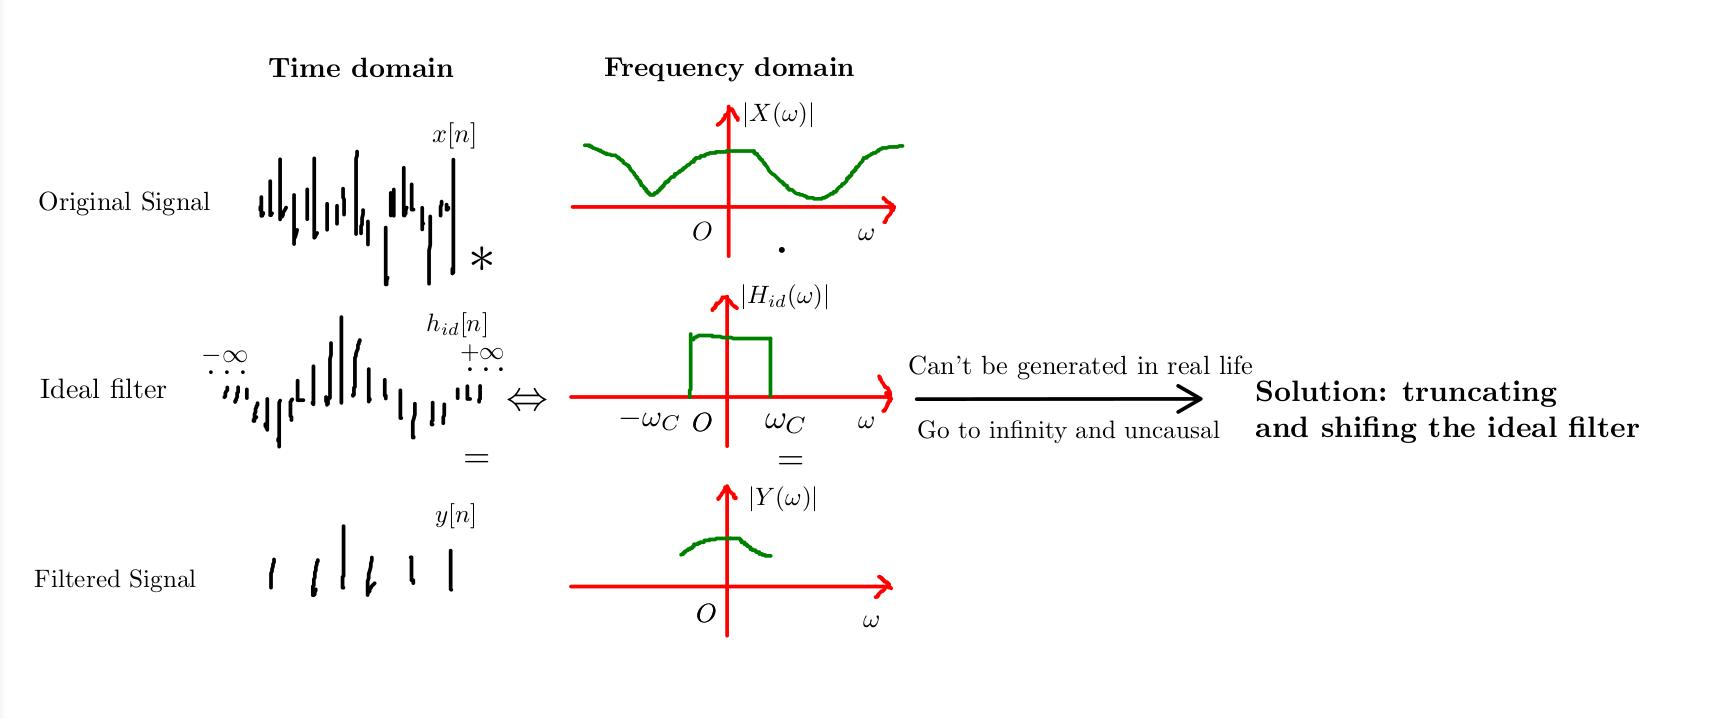
\includegraphics[width=1.1\textwidth]{2.jpg}
		\caption{Ideal filter}			\label{fig:re2}
	\end{figure}
	Từ công thức IDTFT, ta dễ dàng xác định được $h_{id}[n]$:
	$$h_{id}[n]=\frac{1}{2\pi}\int_{2\pi}H_{id}(\omega)e^{j\omega n}d\omega=\frac{1}{2\pi}\int_{-\pi}^{\pi}e^{j\omega n}d\omega=\frac{1}{2\pi}\int_{-\omega_{C}}^{+\omega_{C}}e^{j\omega n}d\omega=\alert{\frac{\sin{\omega_{C}n}}{\pi n}}$$

\end{frame}
\begin{frame}{Ý tưởng thiết kế bộ lọc FIR}
	\begin{figure}[h]
		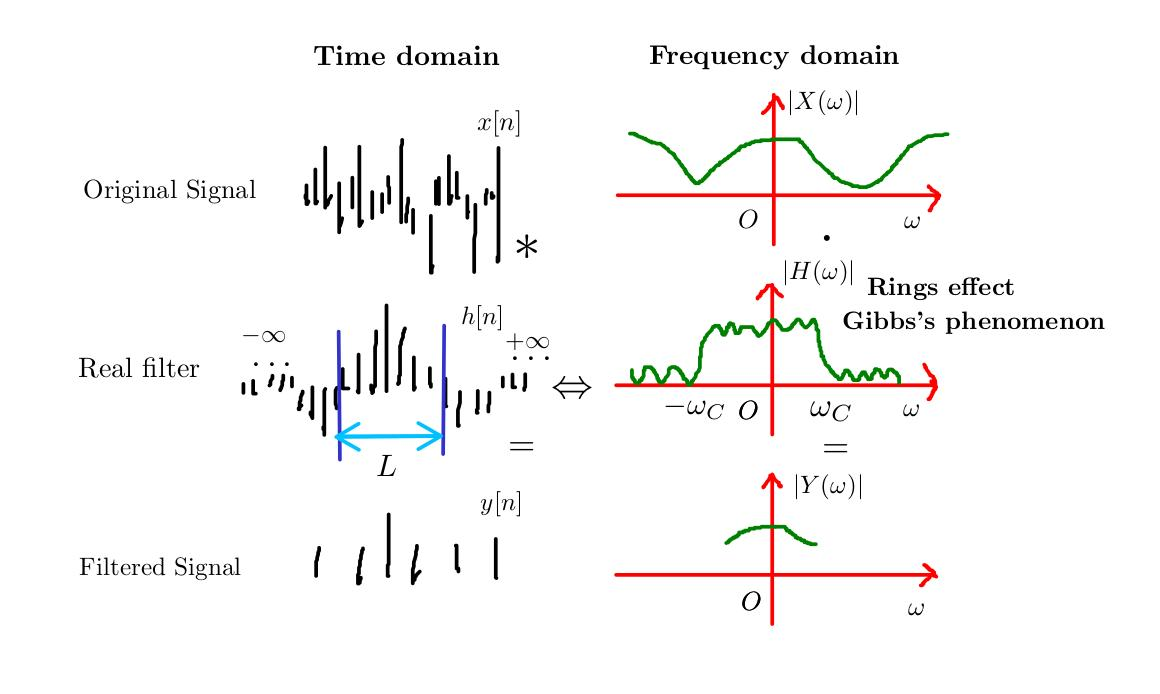
\includegraphics[width=1.1\textwidth]{3.jpg}
		\caption{Real filter}			\label{fig:re3}
	\end{figure}
\end{frame}
\begin{frame}{Ý tưởng thiết kế bộ lọc FIR}
	Từ biểu thức DTFT, ta có thể giải thích hiện tượng Gibbs như sau:
	$$H(\omega)=\sum_{n=-\infty}^{+\infty}h[n]e^{-j\omega n}=\sum_{n=-M}^{+M}h[n]e^{-j\omega n}=h[0]+\sum_{n=1}^{M}h[n](e^{j\omega n}+e^{-j\omega n})$$$$=\alert{h[0]+\sum_{n=1}^{M}2h[n]\cos{(\omega n)}}$$
	Ta có thể thấy rất rõ hệ quả của việc cắt cụt $h_{id}[n]$ thành $h[n]$ là \textbf{tạo gợn sóng mạnh} và \textbf{độ suy hao giảm nhanh} ($A_{id}=+\infty\to A\approx 23\text{dB}$).
	\\ Hiển nhiên nếu $L\to+\infty$ (tức là tăng L càng lớn càng tốt) thì $h[n]\to h_{id}[n]$, chất lượng bộ lọc được cải thiện rõ rệt.
	\\ Thế nhưng, trong nhiều trường hợp thực tiễn, việc tăng $L$ trở nên khó khăn, các nhà toán học đã phát triển các phương pháp "cắt" bộ lọc lý tưởng khác tối ưu hơn "cắt" trực tiếp như trên.
	\\  Phương pháp cắt cụt này được gọi là \alert{phương pháp cửa sổ (windowing method)}, được mô tả qua biểu thức sau: $$h[n]=h_{id}[n]\alert{\cdot}w[n]$$
\end{frame}
\begin{frame}{Ý tưởng thiết kế bộ lọc FIR}
	\begin{figure}[h]
		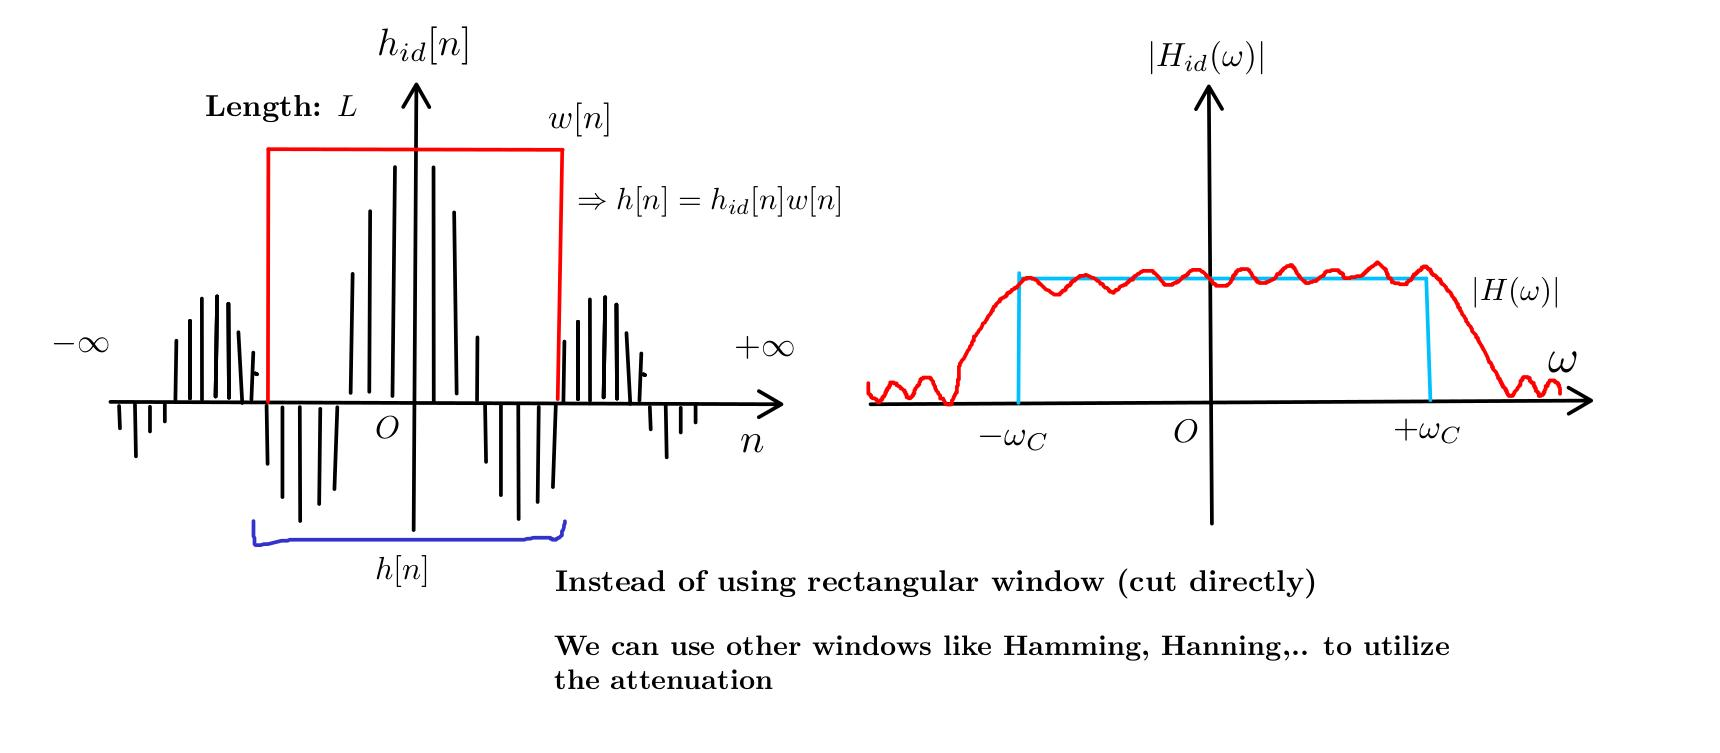
\includegraphics[width=1.1\textwidth]{4.jpg}
		\caption{Windowing method to truncate the ideal filter}			\label{fig:re4}
	\end{figure}

\end{frame}
\begin{frame}{Ý tưởng thiết kế bộ lọc FIR}
	\begin{figure}[h]
		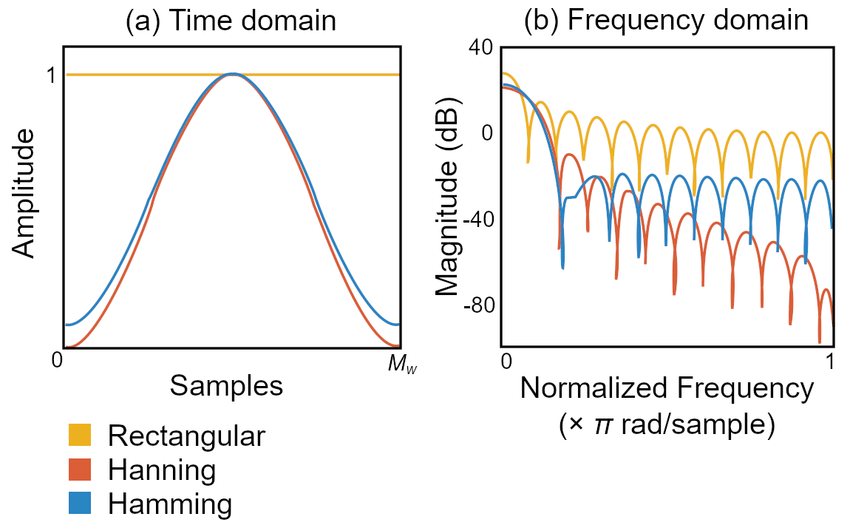
\includegraphics[width=1\textwidth]{The-rectangular-Hanning-and-Hamming-windows-in-the-time-and-frequency-domains-with-Mw.png}
		\caption{Comparing windows in time and frequency domain}			\label{fig:re5}
	\end{figure}
\end{frame}
\begin{frame}{Ý tưởng thiết kế bộ lọc FIR}
	\begin{figure}[h]
		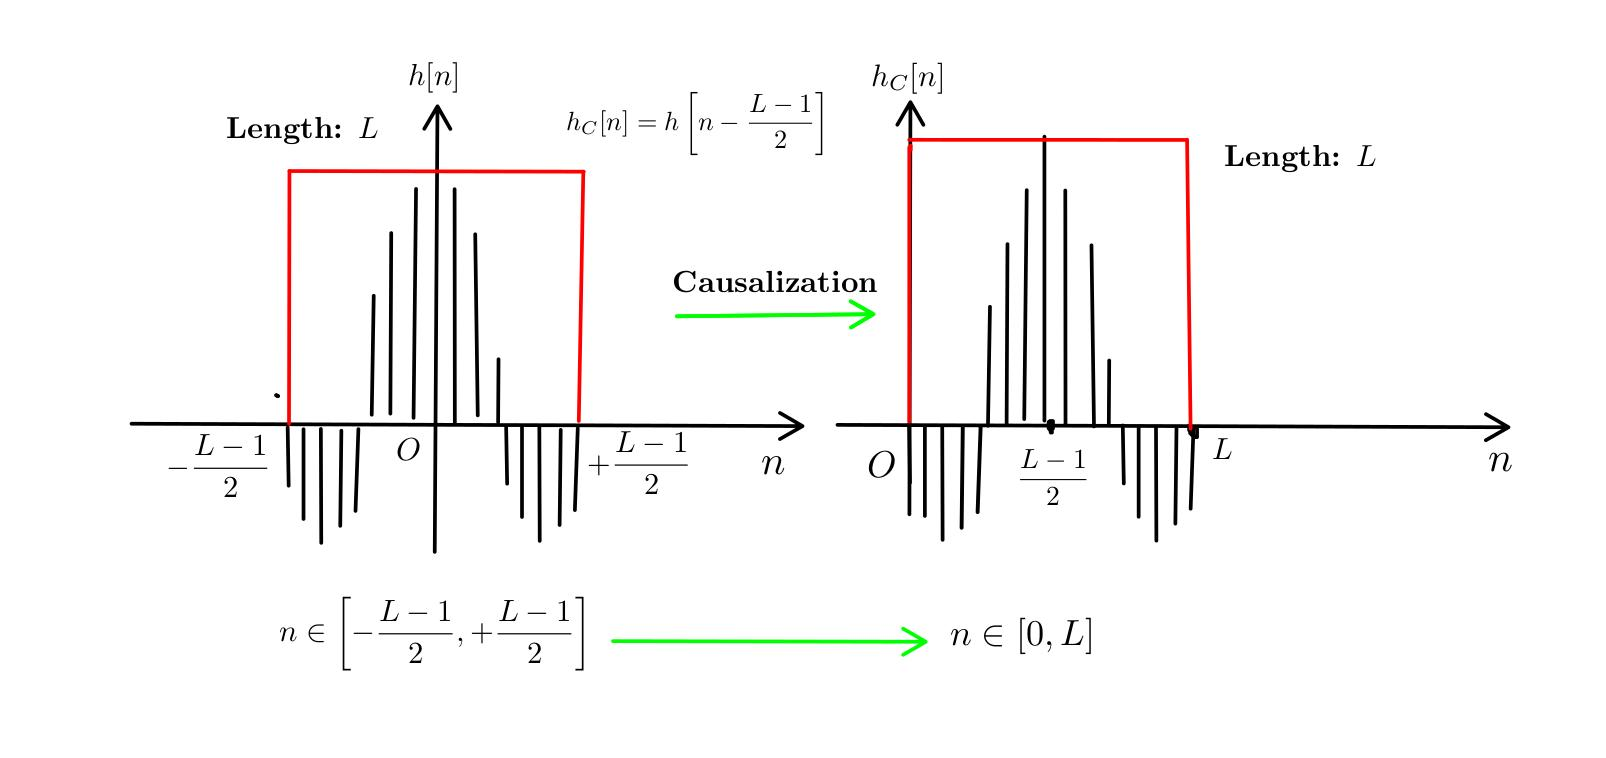
\includegraphics[width=1.1\textwidth]{5.jpg}
		\caption{"Causalization" step}			\label{fig:re6}
	\end{figure}
\end{frame}
\begin{frame}{Thiết kế bộ lọc FIR}
	\section{Thiết kế bộ lọc FIR}
	\subsection{Thiết kế bộ lọc LP}
	\begin{itemize}
		\item Thiết kế bộ lọc LP
	\end{itemize}
	\begin{figure}[h]
		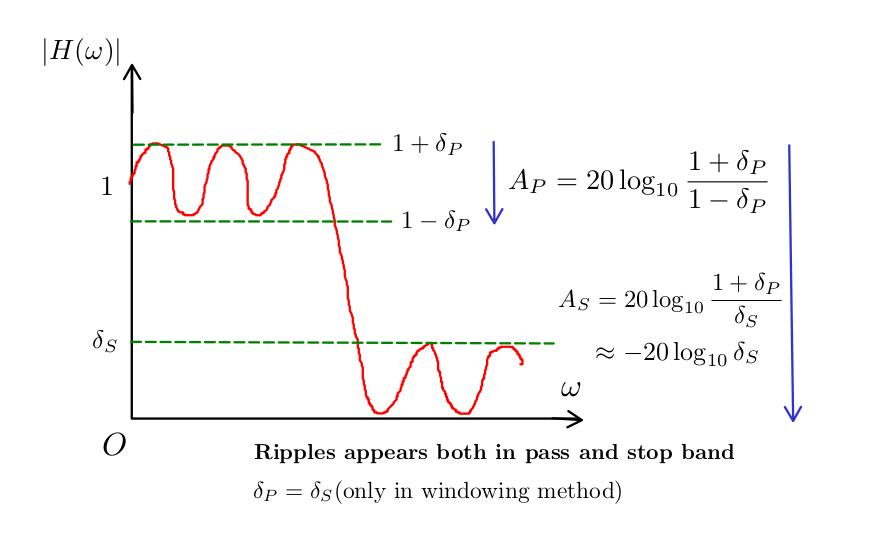
\includegraphics[width=0.9\textwidth]{6.jpg}
		\caption{Frequency response in dB scale}			\label{fig:re7}
	\end{figure}
\end{frame}
\begin{frame}{Thiết kế bộ lọc FIR}
	Ta định nghĩa khái niệm \alert{tần số số} mới như sau:
	$$\alert{v=\frac{F}{F_{sam}}}$$
	\textbf{Lưu ý: khái niệm tần số số (digital frequency) này khác với quy ước của Matlab đã được trình bày rất kĩ ở \alert{Chương 4}}.
	\\ Ta viết lại công thức $h_{id}[n]$ như sau:
	$$h_{id}[n]=\frac{\sin{(\omega_{C}n)}}{n\pi}=2v\frac{\sin{(2\pi v n)}}{2\pi vn}=\alert{2v\text{sinc}(2vn)}$$
	Với: $$\text{sinc(x)}=\frac{\sin{(\pi x)}}{\pi x}$$
	Hiển nhiên từ đáp ứng biên độ trên ta thấy $\Delta v$ và $L$ tỉ lệ \alert{nghịch} với nhau, tức là: $$\Delta v=\frac{C}{L}$$
	\begin{figure}[h]
		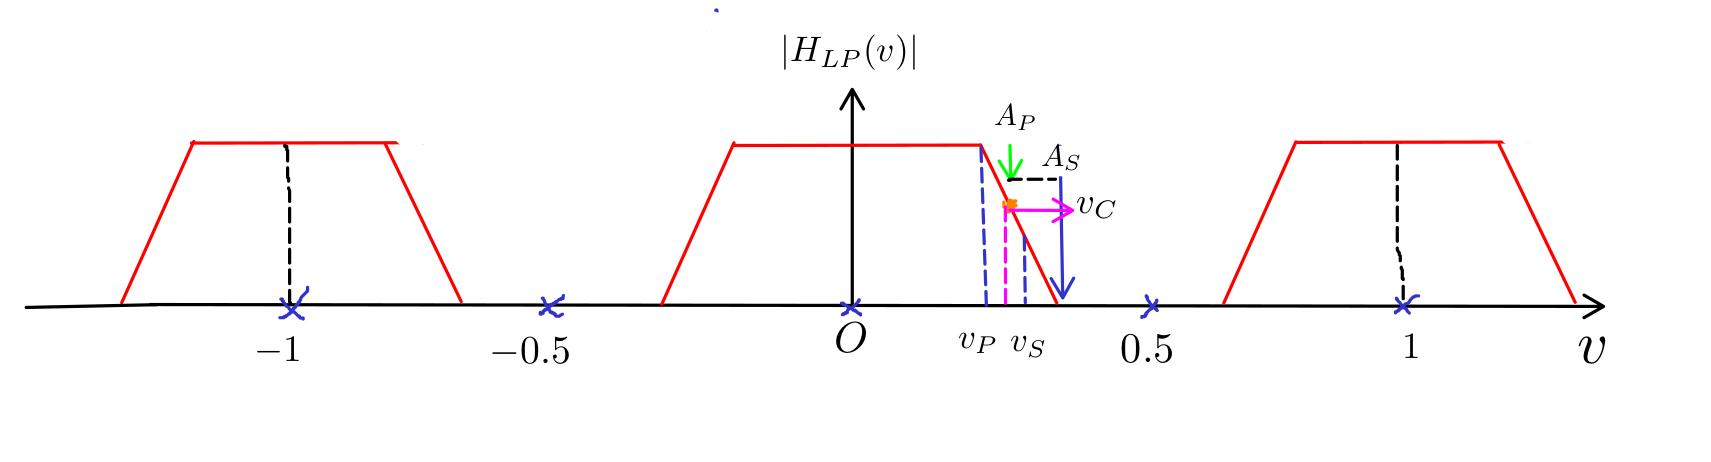
\includegraphics[width=0.7\textwidth]{7.jpg}
		\caption{Designing FIR LP filter}			\label{fig:re8}
	\end{figure}
\end{frame}
\begin{frame}{Thiết kế bộ lọc FIR}
	\begin{block}{Thuật toán thiết kế bộ lọc FIR LP}
		\begin{enumerate}
			\item[1] Quy đổi tần số về \alert{tần số số} (theo quy chuẩn thường):
				$$\alert{v=\frac{F}{F_{sam}}}$$
			\item[2] Xác định tần số số cắt: $$v_{C}=\frac{v_{P}+v_{S}}{2}$$
			\item[3] Chọn cửa sổ $w[n]$ có $A_{w,S}\geq A_{S}$.
			\item[4] Từ cửa sổ đã chọn, xác định chiều dài cửa sổ: $$\Delta v=\frac{C}{L}$$
			\item[5] Thiết kế bộ lọc FIR: $$h[n]=h_{id}[n]w[n]=\alert{2v_{C}\textbf{sinc}(2v_{C}n)w[n]}\quad\left(|n|\leq\frac{L-1}{2}\right)$$
			\item[6] Dịch nhân quả:
				$$h_{C}[n]=h\left[n-\frac{L-1}{2}\right]\quad(0\leq n\leq L-1)$$
		\end{enumerate}
	\end{block}
\end{frame}
\begin{frame}{Thiết kế bộ lọc FIR}
	\begin{figure}[h]
		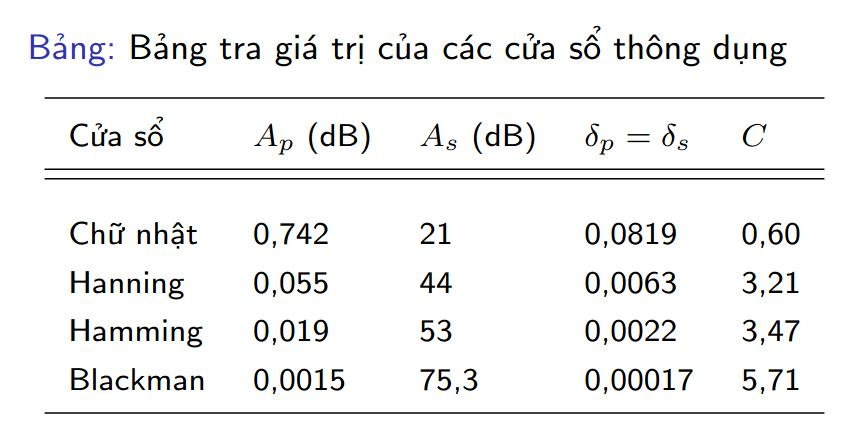
\includegraphics[width=0.8\textwidth]{8.jpg}
		\caption{Windows table}			\label{fig:re9}
	\end{figure}
\end{frame}
\begin{frame}{Thiết kế bộ lọc FIR}
	\begin{figure}[h]
		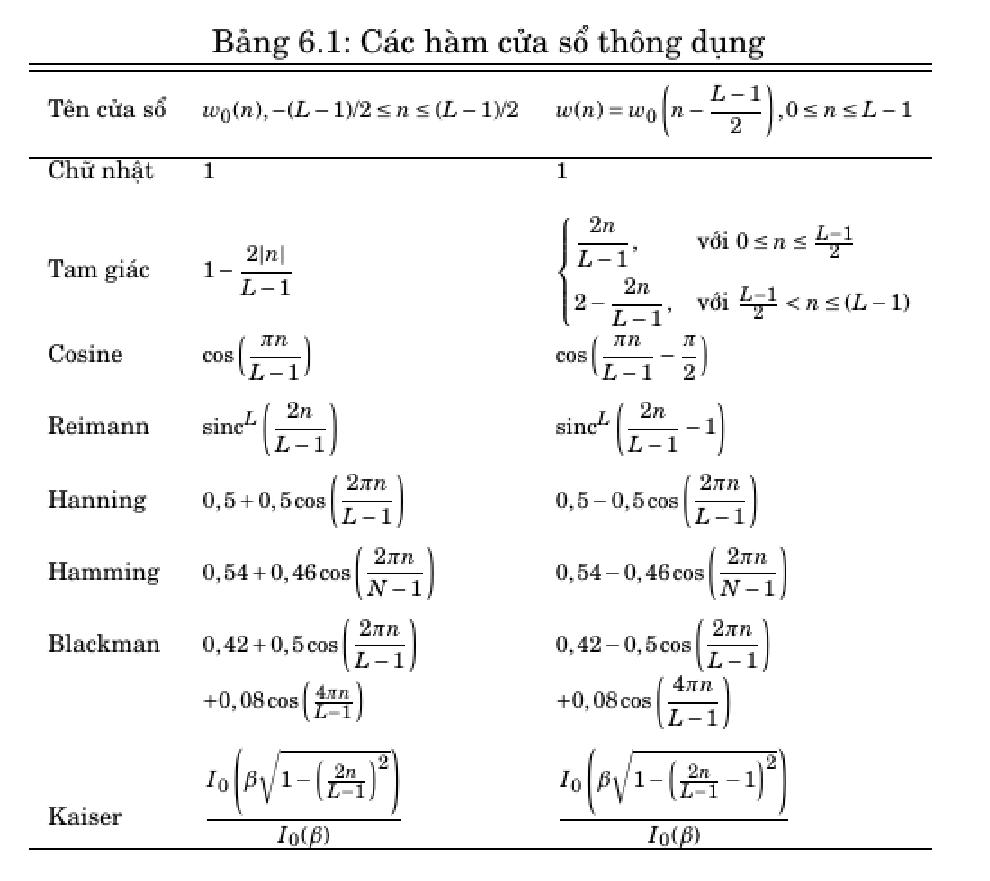
\includegraphics[width=0.8\textwidth]{9.jpg}
		\caption{Windows table}			\label{fig:re10}
	\end{figure}

\end{frame}
\begin{frame}{Thiết kế bộ lọc FIR}
	Ví dụ: thiết kế bộ lọc FIR LP có đặc tả $F_{P}=100\text{Hz},F_{S}=200\text{Hz},F_{sam}=500\text{Hz},$ $A_{P}=2\text{dB},$ $A_{S}=50\text{dB}.$
	\\Từ quy trình thiết kế đã được trình bày rất kĩ ở trên, trước tiên ta đổi toàn bộ tần số sang tần số số:
	$$\alert{v=\frac{F}{F_{sam}}}\Rightarrow v_{P}=0.2,v_{S}=0.4$$
	Dễ dàng suy ra: $$v_{C}=\frac{v_{P}+v_{S}}{2}=0.3$$
	Do $A_{S}=50$dB, nên ta chọn \textbf{cửa sổ Hamming} thỏa mãn $A_{w,S}>50$dB (phương án chọn cửa sổ Blackman có $A_{w,S}=75.3$dB hoàn toàn hợp lý). Tra bảng, ta thấy $C=3.47$.
	\\ Ta tìm được chiều dài cửa sổ $w_{Hamming}[n]$ như sau:
	$$\alert{\Delta v=\frac{C}{L}}\Rightarrow L=\frac{3.47}{0.4-0.2}=17.35$$
	Ta chọn chiều dài cửa sổ $L=19$ để thỏa mãn đặc tả thiết kế.
	\\ Vậy ta dễ dàng suy ra phương trình bộ lọc:
	$$h[n]=w_{Hamming}[n]h_{id}[n]=w_{Hamming}[n]2v_{C}\text{sinc}(2v_{C}n)$$
	$$=0.6w_{Hamming}[n]\text{sinc}(0.6n)\quad\left(|n|\leq 9\right)$$
	Dịch nhân quả, ta thu được:
	$$h_{C}[n]=h[n-9]=0.6w_{Hamming}[n-9]\text{sinc}[0.6(n-9)]\quad(0\leq n\leq 18)$$
\end{frame}
\begin{frame}{Thiết kế bộ lọc FIR}
	\subsection{Thiết kế bộ lọc HP}
	\begin{itemize}
		\item Thiết kế bộ lọc HP
	\end{itemize}
	\begin{figure}[h]
		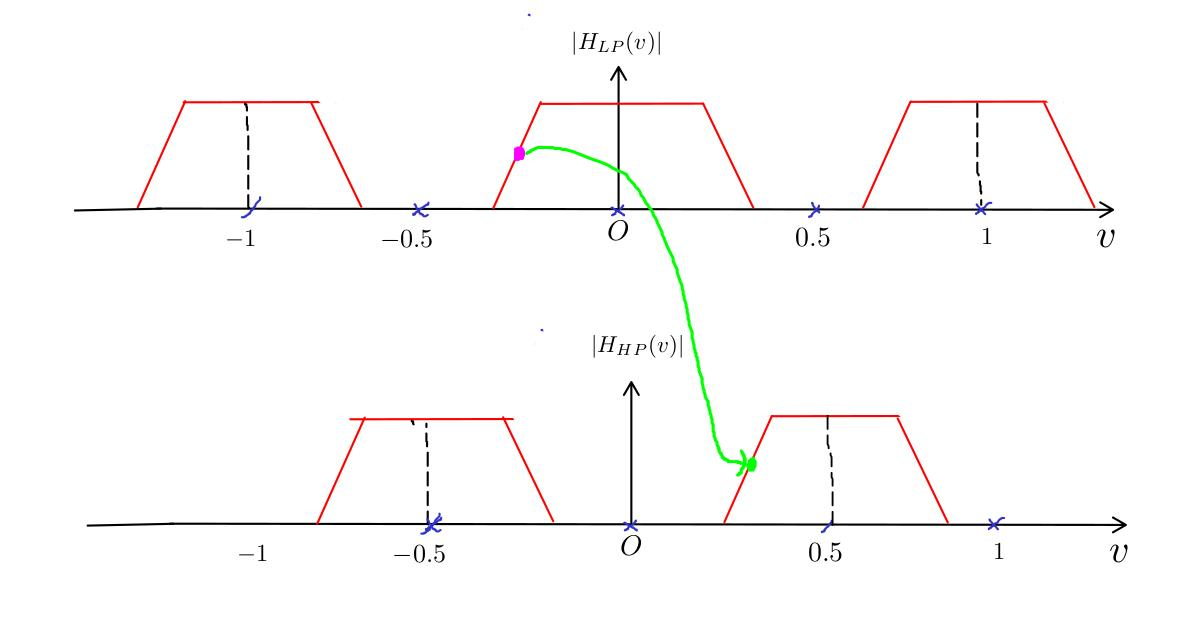
\includegraphics[width=0.8\textwidth]{10.jpg}
		\caption{Designing HP filter}			\label{fig:re11}
	\end{figure}
	Một cách xấp xỉ gần đúng, ta có thể thấy:
	$$|H_{HP}(v)|=|H_{LP}(v-0.5)|$$ $$|H_{HP}(v)|=1-|H_{LP}(v)|$$
	2 công thức xấp xỉ này gợi cho ta 2 hướng thiết kế bộ lọc FIR HP từ bộ lọc FIR LP cho trước.
\end{frame}
\begin{frame}{Thiết kế bộ lọc FIR}
	Từ phương trình dịch phổ:
	$$|H_{HP}(v)|=|H_{LP}(v-0.5)|\Rightarrow h_{HP}[n]=(-1)^{n}h_{LP}[n]$$
	Ta ánh xạ tần số từ bộ lọc LP sang bộ lọc HP, dễ thấy: $$\alert{v_{C}=0.5-\frac{v_{P}+v_{S}}{2}}$$
	Ta xây dựng thuật toán thiết kế bộ lọc FIR HP như sau:
	\begin{block}{Thuật toán thiết kế bộ lọc FIR HP}
		\begin{enumerate}
			\item[1] Quy đổi tần số về tần số số (theo quy chuẩn thường):
				$$\alert{v=\frac{F}{F_{sam}}}$$
			\item[2] Xác định tần số cắt:
				$$\alert{v_{C}=0.5-\frac{v_{P}+v_{S}}{2}}$$
			\item[3] Thiết kế bộ lọc FIR LP với các thông số trên.
			\item[4] Chuyển phương trình đáp ứng xung bộ lọc LP thành HP:
				$$h_{HP}[n]=(-1)^{n}h_{LP}[n] $$
			\item[5] Dịch nhân quả.
		\end{enumerate}
	\end{block}
\end{frame}
\begin{frame}{Thiết kế bộ lọc FIR}
	Từ phương trình phần bù:
	$$|H_{HP}(v)|=1-|H_{LP}(v)|\Rightarrow h_{HP}[n]=\delta[n]-h_{LP}[n]$$
	Tương tự như trên, ta cũng xây dựng một thuật toán khác thiết kế bộ lọc FIR HP như sau:
	\begin{block}{Thuật toán thiết kế bộ lọc FIR HP}
		\begin{enumerate}
			\item[1] Quy đổi tần số về tần số số (theo quy chuẩn thường):
				$$\alert{v=\frac{F}{F_{sam}}}$$
			\item[2] Xác định tần số cắt:
				$$\alert{v_{C}=\frac{v_{P}+v_{S}}{2}}$$
			\item[3] Thiết kế bộ lọc FIR LP với các thông số trên.
			\item[4] Chuyển phương trình đáp ứng xung bộ lọc LP thành HP:
				$$h_{HP}[n]=\delta[n]-h_{LP}[n] $$
			\item[5] Dịch nhân quả.
		\end{enumerate}
	\end{block}
\end{frame}
\begin{frame}{Thiết kế bộ lọc FIR}
	Ví dụ: thiết kế bộ lọc FIR HP có đặc tả $F_{P}=200\text{Hz},F_{S}=100\text{Hz},F_{sam}=500\text{Hz},$ $A_{P}=2\text{dB},$ $A_{S}=50\text{dB}.$
	\\Sử dụng kết quả thiết kế bộ lọc FIR LP trên, ta thu được bộ lọc HP thiết kế bằng phương pháp phần bù:

	$$h_{LP}[n]=0.6w_{Hamming}[n]\text{sinc}(0.6n)\quad\left(|n|\leq 9\right)$$
	$$\Rightarrow h_{HP}[n]=\delta[n]-h_{LP}[n]=\delta[n]-0.6w_{Hamming}[n]\text{sinc}(0.6n)\quad\left(|n|\leq 9\right)$$
	Dịch nhân quả:
	$$h_{C}[n]=h_{HP}[n-9]=\cdots\quad(0\leq n\leq18)$$
	Sử dụng phương pháp dịch phổ, ta phải xác định lại tần số số cắt:
	$$v_{C}=0.5-\frac{v_{P}+v_{S}}{2}=0.5-0.3=0.2$$
	Với cách làm hoàn toàn tương tự, ta thiết kế được bộ lọc FIR LP có đáp ứng xung:
	$$h_{LP}[n]=0.4w_{Hamming}[n]\text{sinc}(0.4n)\quad\left(|n|\leq 9\right)$$
	$$\Rightarrow h_{HP}[n]=(-1)^{n}h_{LP}[n]\quad\left(|n|\leq 9\right)$$
	Dịch nhân quả, ta thu được bộ lọc cần tìm.
\end{frame}
\begin{frame}{Thiết kế bộ lọc FIR}
	\subsection{Thiết kế bộ lọc BP}
	\begin{itemize}
		\item Thiết kế bộ lọc BP
	\end{itemize}
	\begin{figure}[h]
		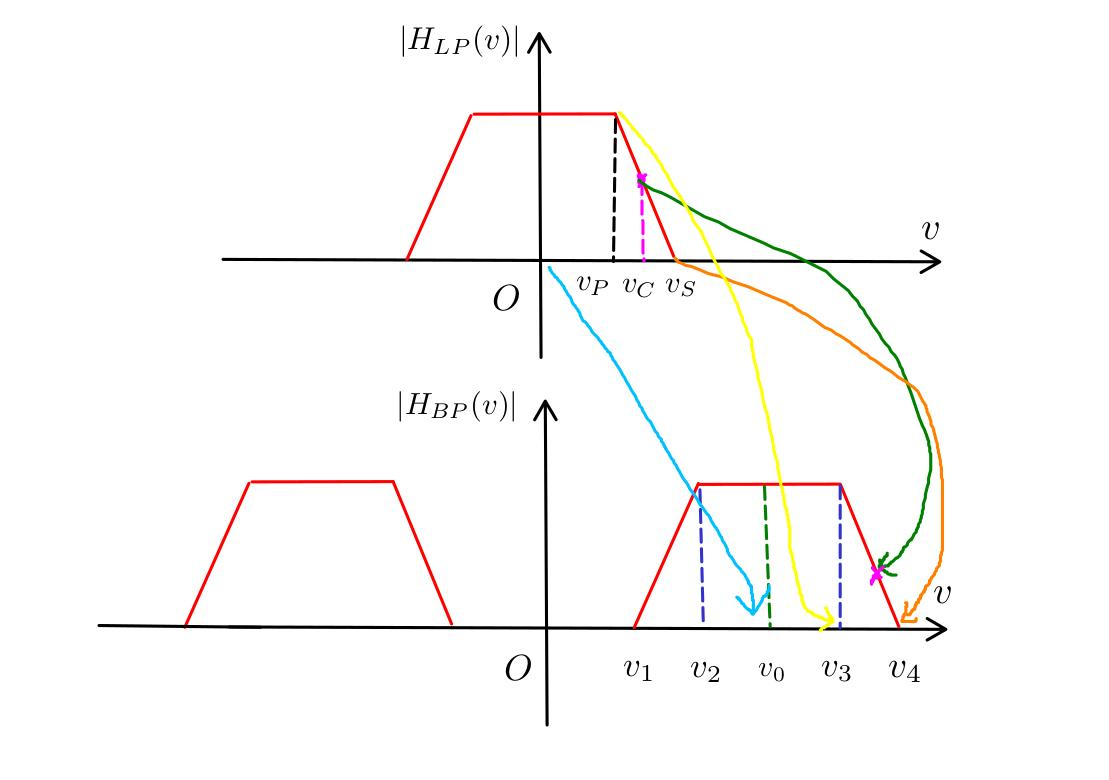
\includegraphics[width=0.8\textwidth]{11.jpg}
		\caption{Designing BP filter}			\label{fig:re12}
	\end{figure}
\end{frame}
\begin{frame}{Thiết kế bộ lọc FIR}
	Ta ánh xạ lần lượt các tần số như hình trên, rất dễ nhìn ra các mối quan hệ hình học:
	\begin{equation*}
		\begin{split}
			v_{0}&=\frac{v_{1}+v_{4}}{2}=\frac{v_{2}+v_{3}}{2}\\
			v_{C}&=\frac{v_{3}+v_{4}}{2}-v_{0}\\
			v_{P}&=v_{3}-v_{0}\\
			v_{S}&=v_{4}-v_{0}\\
		\end{split}
	\end{equation*}
	Hiển nhiên từ dạng phổ ta thấy:
	$$|H_{BP}(v)|=|H_{LP}(v-v_{0})|+|H_{LP}(v+v_{0})|\Rightarrow h_{BP}[n]=2\cos({2v_{0}n})h_{LP}[n]$$
	Vậy ta xây dựng thuật toán thiết kế bộ lọc FIR BP như sau:
\end{frame}
\begin{frame}{Thiết kế bộ lọc FIR}
	\begin{block}{Thuật toán thiết kế bộ lọc FIR BP}
		\begin{enumerate}
			\item[1] Quy đổi tần số $F$ về tần số số $v$ theo quy chuẩn thường.
			\item[2] Xác định các thông số cần thiết của bộ lọc LP bằng công thức sau:
				\begin{equation*}
					\begin{split}
						v_{0}&=\frac{v_{1}+v_{4}}{2}=\frac{v_{2}+v_{3}}{2}\\
						v_{C}&=\frac{v_{3}+v_{4}}{2}-v_{0}\\
						v_{P}&=v_{3}-v_{0}\\
						v_{S}&=v_{4}-v_{0}\\
					\end{split}
				\end{equation*}
			\item[3] Thiết kế bộ lọc LP theo thông số trên.
			\item[4] Chuyển phương trình đáp ứng xung bộ lọc LP thành BP:
				$$h_{BP}[n]=2\cos({2v_{0}n})h_{LP}[n]$$
			\item[5] Dịch nhân quả và thu được bộ lọc cần tìm.

		\end{enumerate}
	\end{block}
\end{frame}
\begin{frame}{Thiết kế bộ lọc FIR}
	Ví dụ: thiết kế bộ lọc FIR BP có đặc tả sau với $F_{sam}=25$kHz:
	$$4\text{kHz}<F<8\text{kHz},A_{P}<3\text{dB}$$
	$$F<2\text{kHz},F>10\text{kHz},A_{S}>45\text{dB}$$

	Quy đổi ra tần số số, ta có:
	$$v_{1}=0.08,v_{2}=0.16,v_{3}=0.32,v_{4}=0.4\Rightarrow v_{0}=0.24,v_{C}=0.12$$
	Ta chọn cửa sổ Hamming với $C=3.47$, suy ra $L=45$.
	\\ Ta rất dễ dàng xác định được: $$h_{LP}[n]=w_{Hamming}[n]h_{id}[n]=w_{Hamming}[n]0.24\text{sinc}(0.24n)$$
	Vậy ta suy ra: $$h_{BP}[n]=2\cos(0.48n)w_{Hamming}[n]0.24\text{sinc}(0.24n)=0.48\cos(0.48n)\text{sinc}(0.24n)$$
	Dịch nhân quả, ta thu được bộ lọc FIR BP cần tìm.
\end{frame}
\begin{frame}[fragile]{Thực hành}
	\section{Thực hành}
	Ta thử phác họa đáp ứng biên độ và khảo sát ảnh hưởng của hiện tương Gibbs với cửa sổ chữ nhật.
	\begin{verbatim}
pkg load signal;
graphics_toolkit("qt");
M=50; % Adjust window length
n=-M:1:M;
F=10;Fs=100;v=F/Fs;
xn=[sin(2*pi*v*n)./(2*v*n*pi)].*(2*v);
xn(n==0)=2*v;
subplot(3,1,1);
stem(n,xn);
title('Rectangular window in time domain');
subplot(3,1,2);
L=length(n);
Xn=fftshift(fft(xn));
Mag_Xn=abs(Xn)/L;
v=linspace(-0.5,0.5,L);
plot(v,Mag_Xn);
title("Rectagular window in frequency domain");
subplot(3,1,3);
plot(v,20*log(Mag_Xn));
title("Rectangular window in dB scale");
pause;
\end{verbatim}
\end{frame}
\end{document}
